%% content.tex
%%

%% ===========================
\chapter{Systemanalyse}
\label{ch:Systemanalyse}
%% ===========================

Zu Beginn der Arbeiten wird eine Systemanalyse zur Ermittlung des Ist- und Sollzustandes durchgeführt. Nach \cite{SWB-380277719} versteht man darunter das Beschreiben der vorhandenen und zukünftigen Systeme. Zuerst wird in Abschnitt \ref{ch:Systemanalyse:sec:genesisWorld} eine Ist-Analyse durchgeführt. In Abschnitt \ref{ch:Systemanalyse:sec:Anforderungsanalyse} wird auf die, an das System gestellt, Anforderungen eingegangen. Aufbauend auf den Anforderungen werden in Abschnitt \ref{ch:Systemanalyse:sec:Information} die relevanten Daten für die Umsetzung ermittelt. 

%% ===========================
\section{CAS genesisWorld}
\label{ch:Systemanalyse:sec:genesisWorld}
%% ===========================

CAS genesisWorld ist eine Software, die Organisation und Zusammenarbeit in Kundenbeziehungen und zwischen Kollegen steigern soll. Alle Informationen bzw. Daten werden in CAS genesisWorld zentral gespeichert und sind so für alle verfügbar. Welche Daten ein Anwender sieht, hängt von seinen Rechten und Einstellungen ab. Die Daten, d.h. Termine, Aufgaben, Adressen, Dokumente usw. werden in CAS genesisWorld von den Nutzern gepflegt und aktuell gehalten. Darüber hinaus lassen sich wie in Abbildung \ref{picGwCon} dargestellt, alle Daten beliebig miteinander verknüpfen. So werden zusätzliche Zusammenhänge deutlich und der Informationsgehalt steigt. Ein Besprechungstermin lässt sich beispielsweise mit den Adressen der Teilnehmer und dem Dokument der Tagesordnung verknüpfen.

\begin{figure}[H]
	\centering
  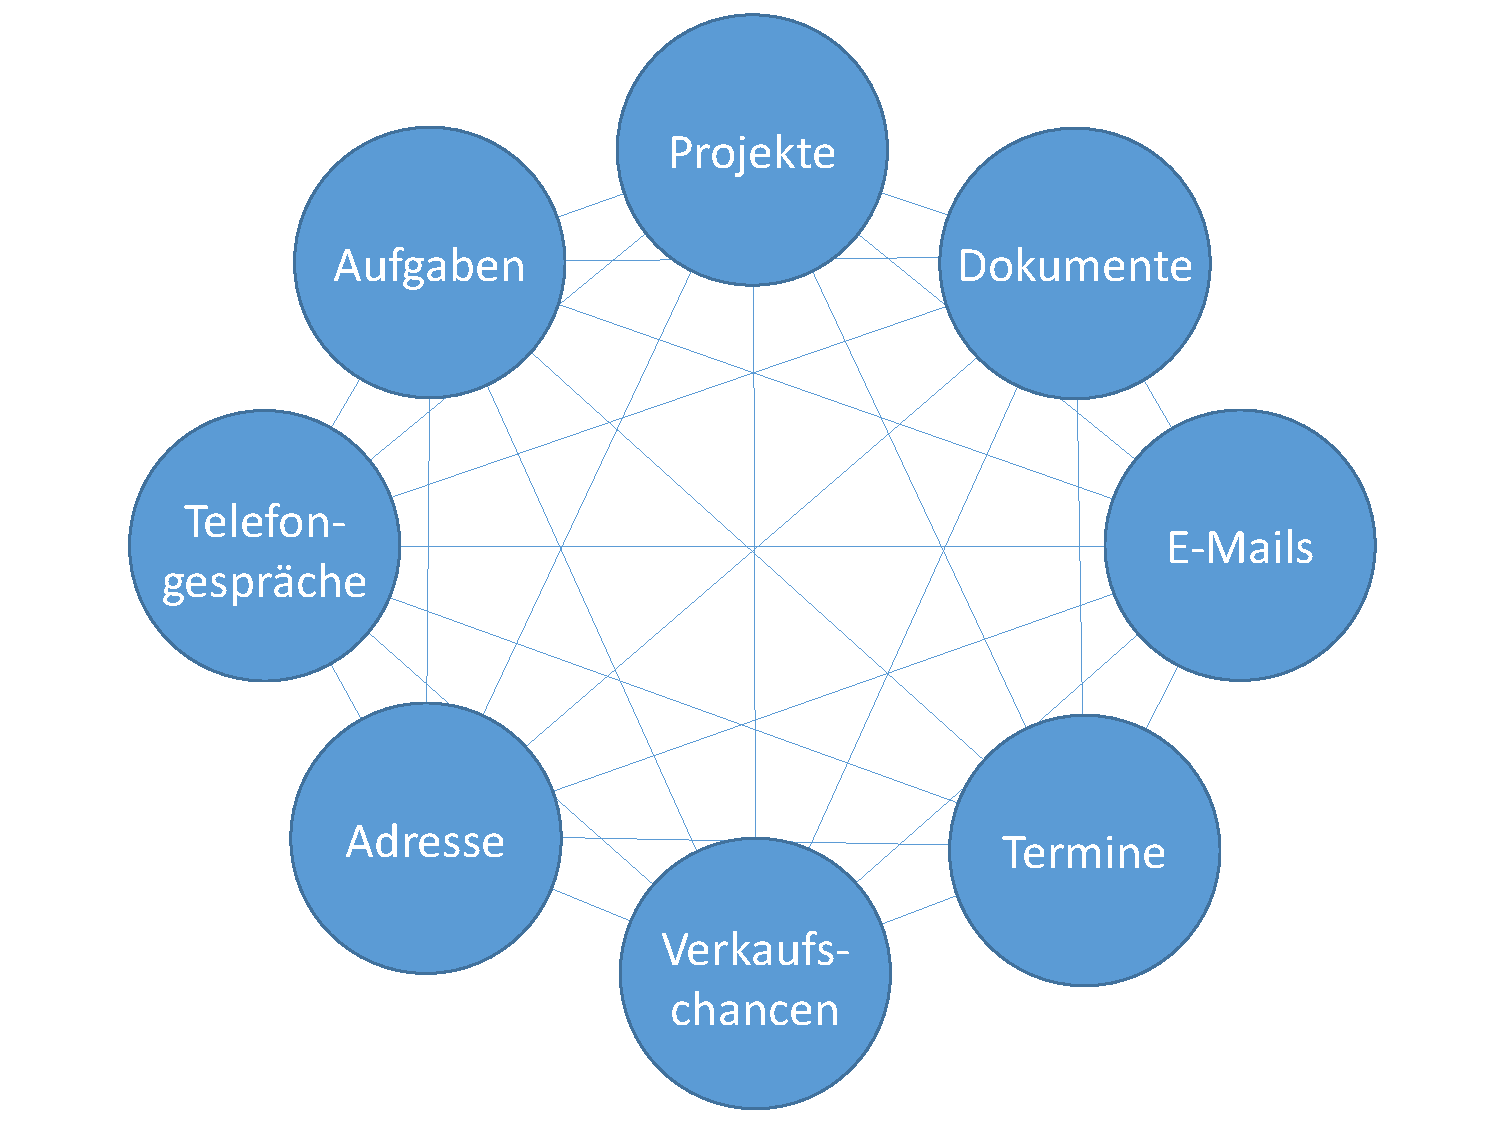
\includegraphics[width=0.5\textwidth, width=0.5\textwidth]{pics/CAS_connections.pdf}
	\caption{Verknüpfungen in CAS genesisWorld}
	\label{picGwCon}
\end{figure}

%% ===========================
\subsection{Architektur}
%% ===========================

Die N-Tier-Architektur von CAS genesisWorld lässt sich in drei wesentliche Bereiche gliedern:

\begin{itemize}

	\item Die Präsentationsclients umfassen alle Dienste, die Informationen in Bildschirmansichten den Benutzern zur Verfügung stellen.
	
	\item Der Applikationsserver umfasst alle Dienste, um die Geschäftslogik zu kapseln, Änderungen zu protokollieren, Benutzerrechte zu prüfen und die aufbereiteten Informationen den Präsentationsdiensten zur Verfügung zu stellen.
	
	\item Die Datenbankschicht umfasst alle Dienste die zur Datenhaltung selbst notwendig sind.
\end{itemize}


%% ===========================
\subsection{Präsentationsschicht \& Logikschicht}
%% ===========================

Der CAS genesisWorld Client existiert in Form einer Windowsanwendung, als mobile Version in Android, Windows Phone, BlackBerry OS und iOS. Die Kommunikation der Clients mit CAS genesisWorld findet über das REST-Protokoll statt \cite{cas2013a}.

Die Funktionalität des CAS genesisWorld Anwendungsservers wurde in Form von COM-Objekten implementiert. Damit stehen dessen Dienste auch Dritten zur Verfügung, die dadurch mit eigenen Applikationen die Informationen von CAS genesisWorld präsentieren oder weiterverarbeiten können. Eine erster Überblick der CAS genesisWorld Komponenten ist in Abbildung \ref{gw_Architektur} zu sehen. Als Basisdienste stehen der UserService und der DataService zu Verfügung. Für die Anmeldung und Rechteverwaltung ist der UserService zuständig. Der DataService ist als zentraler Dienst für den Zugriff auf die CAS genesisWorld Daten verantwortlich. Die Schnittstelle des DataService wurde an Microsoft ADO angelehnt. Auf den Basisdiensten aufbauend existieren die Geschäftsdienste, in Form der Schnittstellen der BusinessServices. Diese bieten spezielle Funktionen zu den jeweiligen Anwendungsbereichen.

\begin{figure}[H]
	\centering
  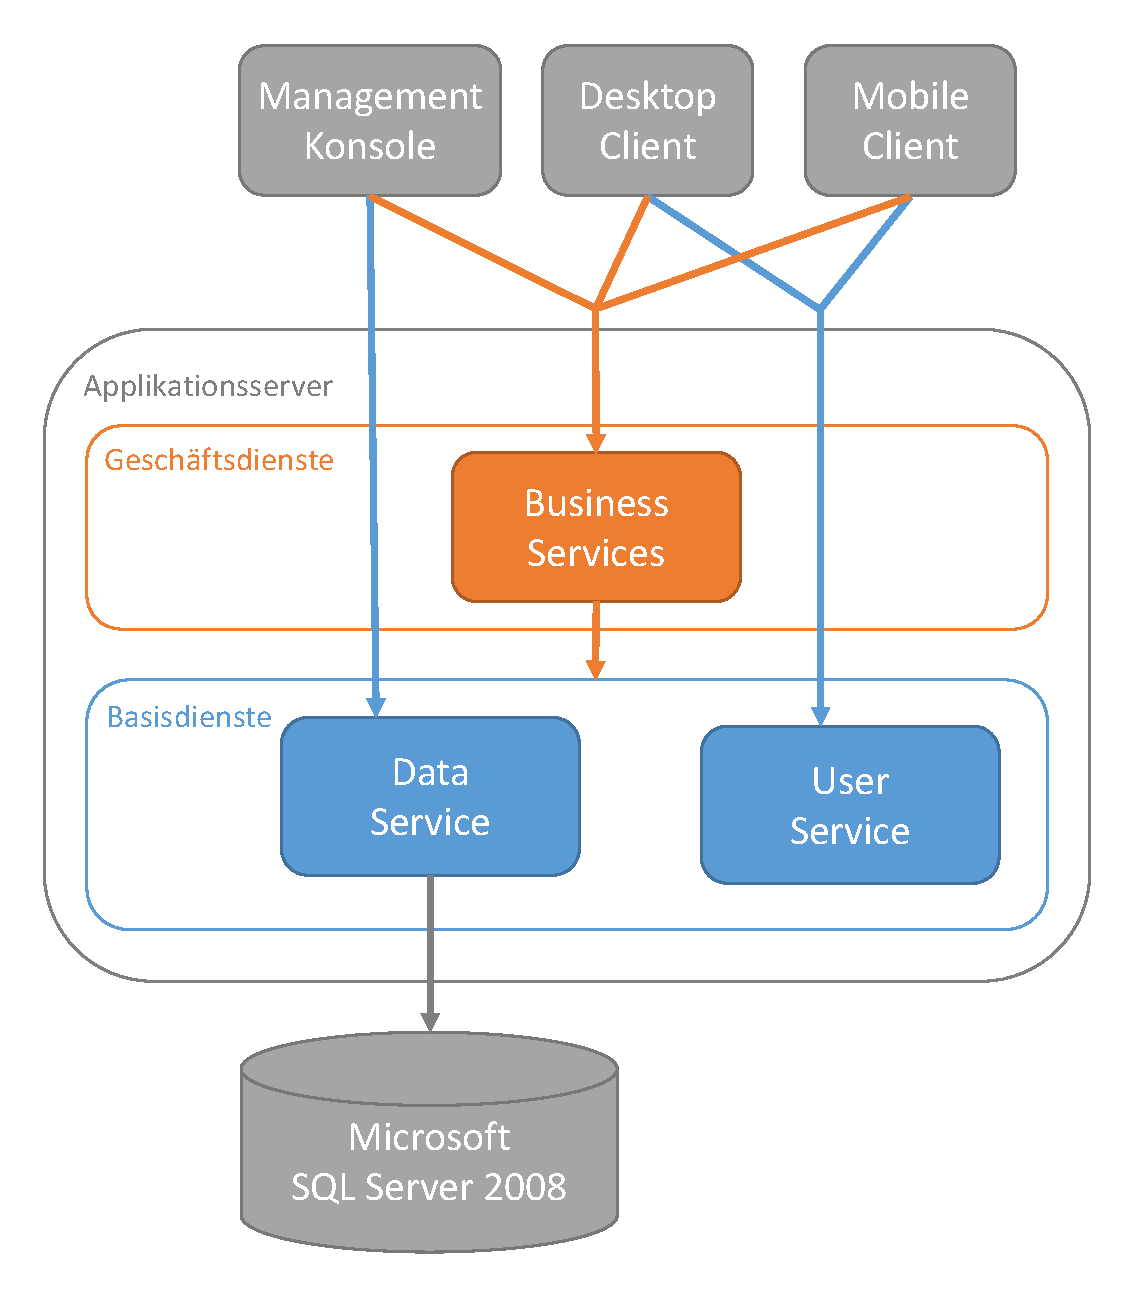
\includegraphics[width=0.6\textwidth, width=0.6\textwidth]{pics/GenesisWorld_Architektur.pdf}
	\caption{Schematische Darstellung der Architektur von CAS genesisWorld}
	\label{gw_Architektur}
\end{figure}

%% ===========================
\subsection{Server-SDK-Plugin}
\label{ch:Systemanalyse:sec:genesisWorld:subsec:plugin}
%% ===========================

Die Server-SDK-Plugins bieten die Möglichkeit die Datenverarbeitung, um eine eigene Logik zu erweitern oder zu modifizieren. 

Realisiert werden die Plugins als COM-Objekte, die ein Plugin-Interface namens \textit{IGWSDKDataPlugIn} implementieren. Das erstellte COM-Objekt wird im Server von CASgenesisWorld registriert. Der Server delegiert bei einer Datenoperation den Aufruf an die für den jeweiligen Datensatztypen registrierten Plugins. In Abbildung \ref{gw_plugin} ist ein Beispiel des Vorgangs dargestellt. Die CASTable ist für die Delegation der Datenmanipulation-Anweisungen zuständig. Sie empfängt Anweisungen vom DataService und führt diese auf dem MSSQL-Server aus. Außerdem besitzt sie mit dem Plugin-Direktor eine Komponente mit der Plugins über Änderungen in den Datensätzen informiert werden. Wie in der Abbildung zu sehen werden zuerst die fest integrierten Plugins wie das CAS-Address-Plugin benachrichtigt. Anschließend werden die von Dritten erstellten Plugins informiert.

\begin{figure}[H]
	\centering
  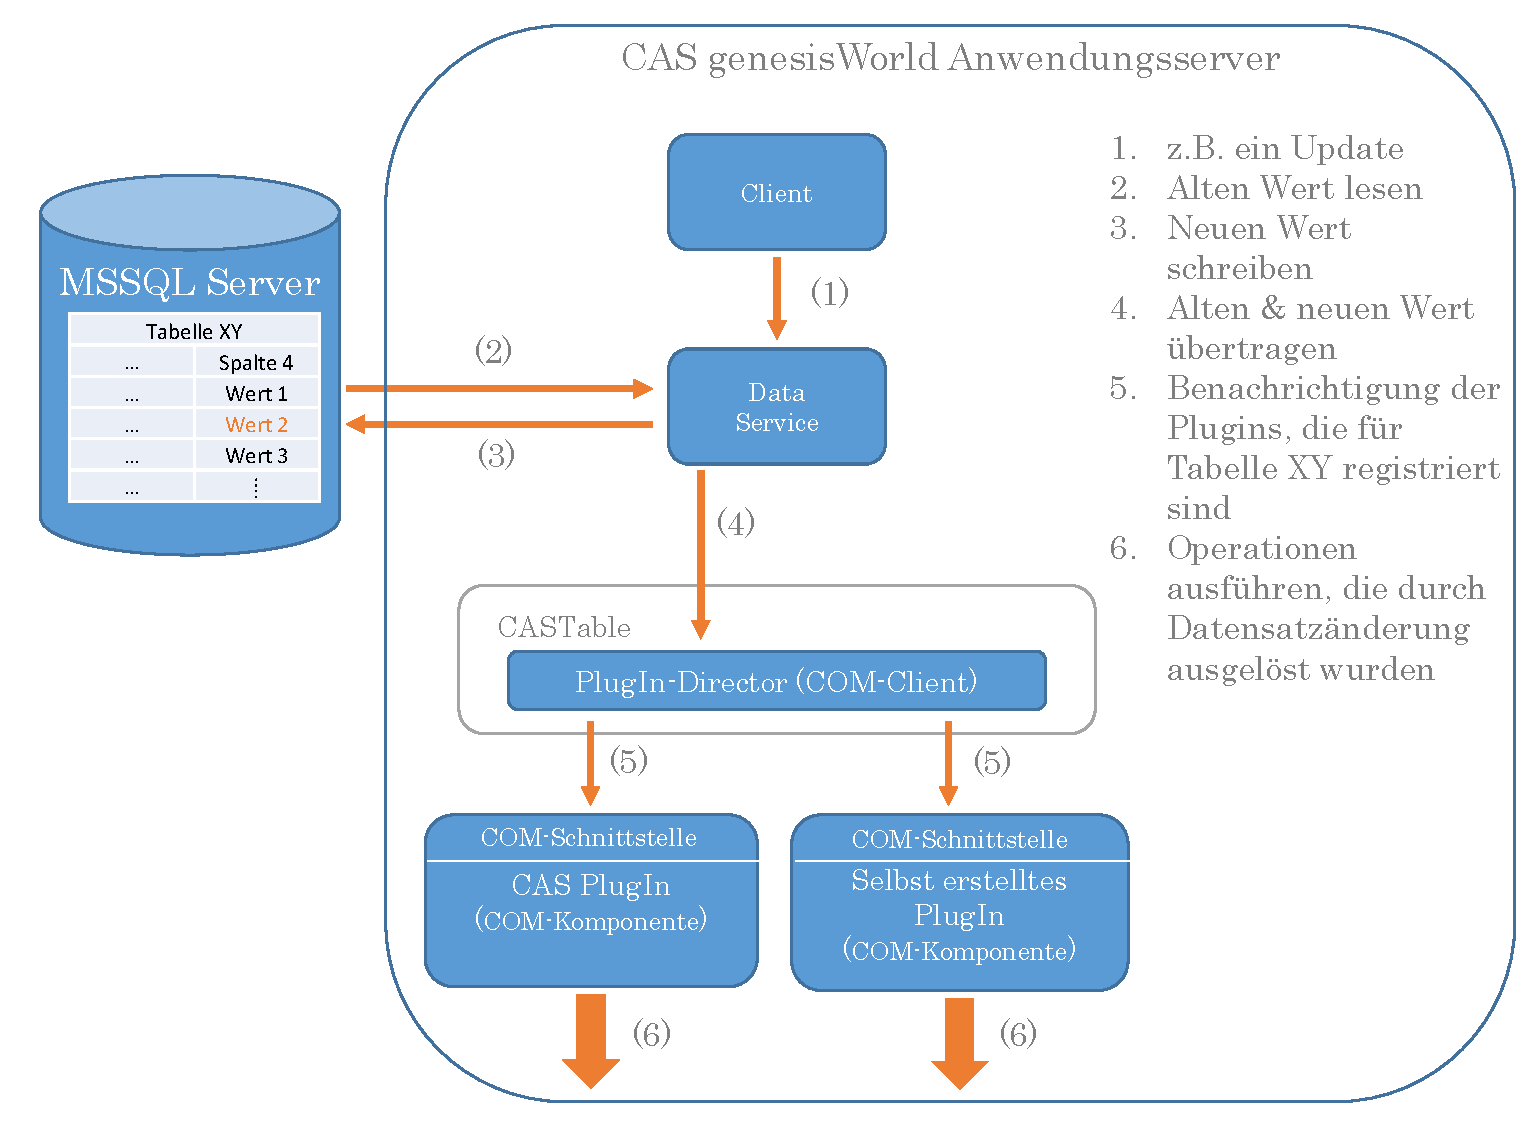
\includegraphics[width=1.0\textwidth, width=1.0\textwidth]{pics/analyse_plugins.pdf}
	\caption{Beispiel zur Benachrichtigung von Plugins anhand eines Ablaufs bei einem Update}
	\label{gw_plugin}
\end{figure}

Im Allgemeinen stehen in den COM-Schnittstellen der Plugins, jeweils alle Felder eines Datensatztypen zur Verfügung, sowie die neuen Werte der Felder. In den Plugins besteht somit die Möglichkeit, alte bzw. neue Werte von Feldern zu untersuchen und zu vergleichen und auf das Ergebnis zu reagieren.

Die Werte des aktuell verarbeiteten Datensatzes können verändert, d.h. erweitert oder reduziert werden. Darüber hinausgehend sind auch automatisierte Aktionen realisierbar, die weitere Datensätze betreffen. So könnten z.B. abhängig von den Eingangswerten einer neu angelegten Adresse, neue Aufgaben angelegt und mit Inhalt versehen werden. Einige automatische Datenoperationen von CAS genesisWorld werden über CAS-Plugins realisiert, die mit den SDK-Plugins verwandt sind.

%% ===========================
\subsection{Datenhaltungsschicht}
\label{ch:Systemanalyse:sec:genesisWorld:subsec:db}
%% ===========================

Die Datenhaltungsschicht enthält einen Microsoft SQL Server 2008 (MSSQL). Der SQL Server ist ein relationales Datenbankmanagementsystem (RDBMS) von Microsoft, dass für den Einsatz im Konzernumfeld konzipiert wurde. MSSQL verwendet T-SQL (Transact-SQL), eine Erweiterungen von Sybase und Microsoft, die den SQL-Standard um prozedurale Sprachelemente erweitert \cite{tech2013}. Weiterhin unterstützt MSSQL standardisierte Datenbankschnittstellen, wie Open Database Connectivity (ODBC) und Java Database Connectivity (JDBC).

Zunächst wird auf das Schema der Datenbank eingegangen. Dabei wird nicht das gesamte Schema erläutert sondern nur relevante Teile näher betrachtet.    

In relationalen Datenbanken werden Beziehungen über Primär- und Fremdschlüssel abgebildet. Dies ist auch in der MSSQL-Datenbank der Fall, jedoch mit einer Besonderheit. In der MSSQL-Datenbank werden nur Primärschlüssel deklariert. Die Fremdschlüssel sind vorhanden aber nicht als solche markiert. 

Auf die Table Relation eingehen

\textit{TableRelation} 


Abbildung \ref{gw_2} zeigt eine beispielhafte, schematische Darstellung der \textit{TableRelation}.

\begin{figure}[ht]
	\centering
  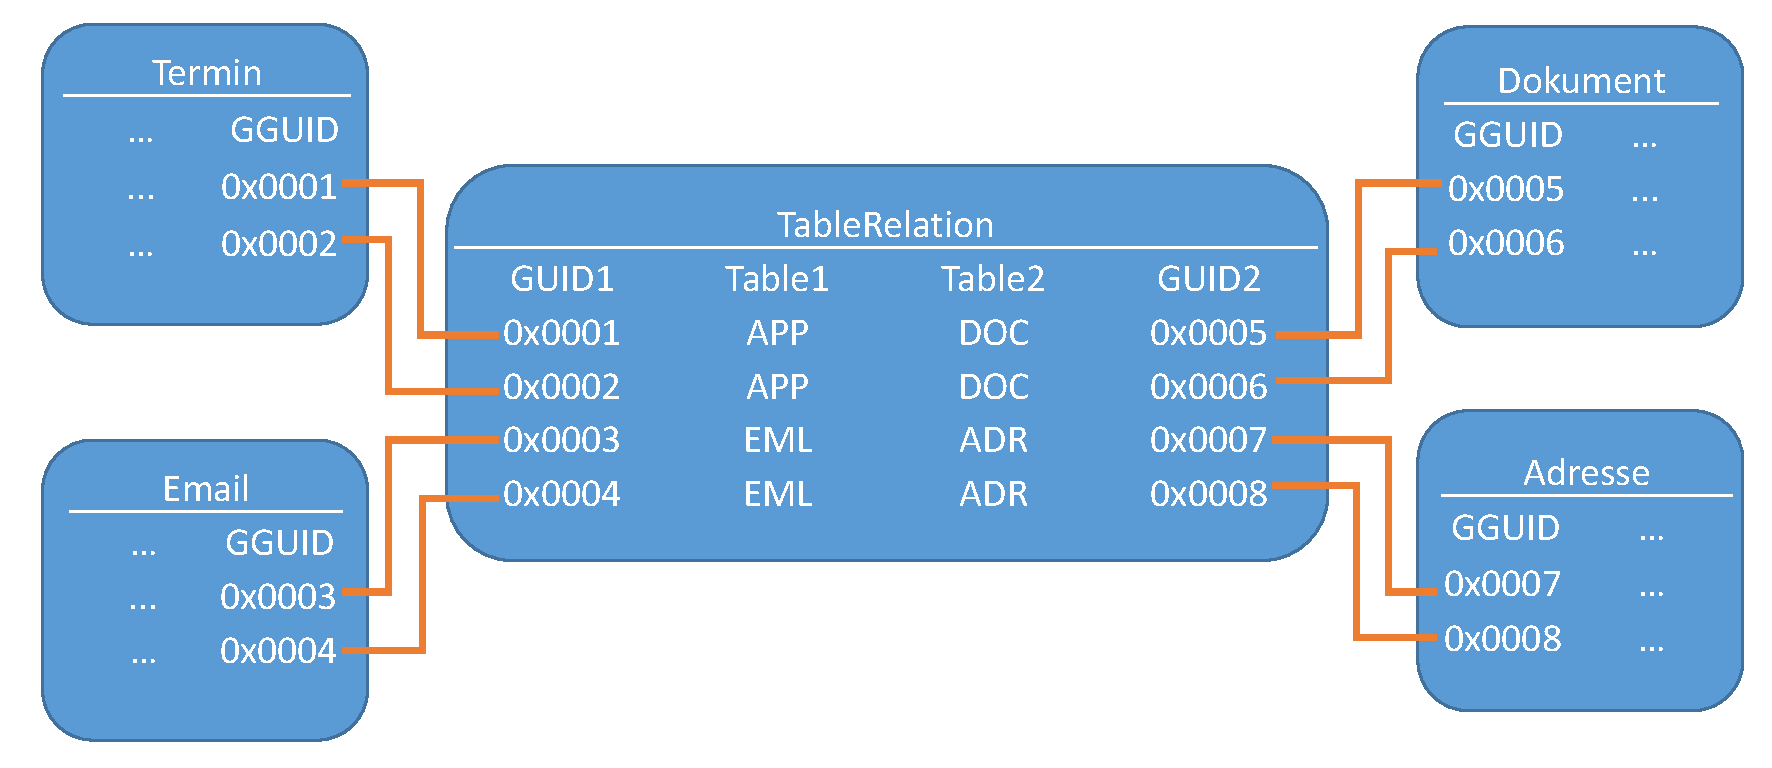
\includegraphics[width=0.9\textwidth, width=0.9\textwidth]{pics/gW_tablerealtion.pdf}
	\caption{Funktionsweise der \textit{RelationTable} anhand eines Beispiels}
	\label{gw_2}
\end{figure}

Die Spalten \textit{GUID1} und \textit{GUID2} beinhalten die jeweiligen Primärschlüssel der in Beziehung zu setzenden Tabellen. Mithilfe der Spalten \textit{TableSign1} und \textit{TableSign2} können die \textit{GGUID}s den Tabellen, aus denen sie entstammen, zugeordnet werden. Die \textit{GGUID} ist in der gesamten Datenbank eindeutig und dient als Primärschlüssel für jede Tupel in der Datenbank.

%% ===========================
\section{Anforderungsanalyse}
\label{ch:Systemanalyse:sec:Anforderungsanalyse}
%% ===========================

Während der Anforderungsanalyse wird ermittelt, welche Eigenschaften und Fähigkeiten das System zur Erreichung der Ziele benötigt. Bei der Einteilung der Anforderungen wird zwischen Funktionalen und Nichtfunktionalen unterschieden. Bei ersterem wird die Funktionalität des zu erstellenden Systems beschrieben, wohingegen alle anderen Anforderungen unter letzteres Fallen. 

%% ===========================
\subsection{Funktionale Anforderungen}
%% ===========================

Bevor wir auf die funktionalen und nichtfunktionalen Anforderungen eingehen, wird das umzusetzende Szenario näher beschrieben. Mit dem zu entwickelndem System soll eine Bewertung der Beziehung zwischen Personen aus CAS genesisWorld ermöglicht werden. Indessen soll ermittelt werden, welche Personen die ausgeprägteste Beziehung zu einer vorher bestimmten Person besitzen. Die Bewertung der Ausprägung basiert auf der Anzahl von Kontakten zwischen den Person. Ein Kontakt wird dabei anhand von fünf verschiedenen Merkmalen ermittelt. Zu einem wird der E-Mail-Verkehr unter den Personen für die Betrachtung herangezogen. Überdies werden in der Bewertung Telefonate zwischen Personen beachtet. Außerdem spielen nachvollziehbare Treffen (Termine) zwischen den Personen eine Rolle. Zwischen Personen geteilte Dokumente werden auch als Merkmal festgesetzt. Das letzte Merkmal ist die Verkaufschance gegenüber einem Kunden. Wie ausgeprägt letztendlich die Beziehung zu einer anderen Person ist, wird anhand der Anzahl solcher Merkmale ermittelt. Auf die fünf Merkmale wird im weiteren Verlauf der Arbeit nur noch mit dem Begriff "Verbindungsmerkmale" verwiesen. Weiterhin ist die Betrachtung nicht auf die gesamte Dauer des Kontakts vorgesehen, sondern auf festgelegte Zeitspannen. Beispielsweise sollten die Ergebnisse auf den Zeitraum vom 01.02 bis 10.08.2013 eingrenzbar sein. Zusätzlich sollten weitere Eingrenzungen möglich sein, die im folgenden Abschnitt beschrieben werden.

Folgende funktionale Anforderungen wurden erhoben:

\begin{itemize}
\item Das System soll die Anzahl von Verbindungsmerkmalen zwischen Personen ermitteln können

\item Das Abfrageergebnis soll eine Rangordnung unter den Personen besitzen und auf der Summe von Verbindungsmerkmalen basieren

\item Das Abfrageergebnis soll die Summe der gesamten Verbindungsmerkmale zu den jeweiligen Person enthalten sowie die Summe der einzelnen Verbindungsmerkmale

\item Benutzer sollen das Abfrageergebnis auf eine bestimmte Anzahl von Personen eingrenzen können

\item Der Zeitraum soll durch den Benutzer beliebig eingrenzbar sein

\item Suchkriterien sollten durch den Benutzer ein- und ausgeblendet werden können, ohne eine neue Abfrage senden zu müssen

\item Gewichtung der Verbindungsmerkmale durch den Nutzer

\item Gewichtung von Zeitspannen durch den Nutzer

\item Filterung der Ergebnismenge durch:	
	\begin{itemize}
	\item Ausschließen von Personen oder Eingrenzen auf Personen
	\item Städte und/oder Länder der Personen
	\item Verringern auf Personen, die einem Unternehmen zugeordnet sind 
	\item Beschränken auf Kontaktpersonen von Unternehmen
	\item Begrenzen auf Kontaktpersonen die keinem Unternehmen angehören
	\item Vermindern um Personengruppen
	\end{itemize}
\end{itemize}

%% ===========================
\subsection{Nichtfunktionale Anforderungen}
%% ===========================

Folgende nichtfunktionale Anforderungen wurden erhoben:

\begin{itemize}
	
	\item Eine Rechnerinstanz für Datenbankserver und Applikationsserver 
	
	\item Sehr kurze Antwortzeiten (< 1s)
	
	\item Lose Kopplung (zwischen Logik und Darstellung)
	
	\item Portabilität
	
	\item Graphische Darstellung des Ergebnisses
	
	\item Keine zusätzliche Kosten

\end{itemize}

%% ===========================
\section{Ermittlung relevanter Daten}
\label{ch:Systemanalyse:sec:Information}
%% ===========================

Die Datenbank der CAS Software AG umfasst 398 Tabellen, die zusammen wiederum 11.620 Spalten beinhalten. Aufgrund einer fehlenden Dokumentation über die Umsetzung der Anwendungsschicht und Beziehungen nicht über Fremdschlüssel identifiziert werden können wurde ein eigenes Verfahren zur Ermittlung von Beziehungen entwickelt. 

Für den Ausgangspunkt der Suche wurde eine Tabelle namens \textit{SysUser} verwendet. Sie beinhaltet jeden Benutzer des Systems. Ihre Eignung beruht auf der Annahme, dass bei der Bewertung von Beziehungen zwischen Personen, die Person selbst den Ausgangspunkt der Suche darstellt. Daher wird zuerst eine Tupel der \textit{SysUser} Tabelle mit ihrer \textit{GGUID} herangezogen. Die \textit{GGUID} ist der erste Wert nachdem in der gesamten Datenbank gesucht wird. Sobald alle Tabellen gefunden wurden, die den Wert beinhalten, wird eine \textit{GGUID} aus jeder Tabelle für die weitere Suche verwendet. Die Anzahl der zu durchsuchenden Tabellen werden nach jedem Schritt um die bereits gefundenen Tabellen verringert. Die Suche wird abgebrochen, sobald die Suchmenge keine Werte mehr aufweist oder keine Tabellen mehr mit den entsprechenden Werten gefunden wurden. Durch dieses Vorgehen werden alle Beziehungen ermittelt, die durch Verwendung der \textit{GGUID} als Referenzwert identifiziert werden können. In Abbildung \ref{gw_schema_alt} ist ein auf das Wesentliche reduzierter Ausschnitt des Ergebnisses zu sehen. 

Von den ursprünglichen 398 Tabellen sind nur noch 17 übrig geblieben, auf die im weiteren Verlauf eingegangen wird. Alle Tabellen enthalten in der ursprünglichen Form wesentlich mehr Spalten und wurden der Übersicht halber entfernt. Tabelle \textit{SysUser} besitzt drei Spalten die von Bedeutung sind. Eine davon ist die \textit{GGUID}, die im Folgenden nicht weiter erwähnt wird, da sie jede Tabelle enthält. Die \textit{OID} wird für jeden Nutzer einmalig vergeben und wird in anderen Tabellen als Zuordnungsmerkmal verwendet. \textit{LoginName} ist der Benutzername des Nutzers und kann beim Anmelden auf der Oberfläche verwendet werden. 

Um Personen aus bestimmten Gruppen aus der Abfrage auszuschließen werden die Tabellen \textit{SysGroupMember} und \textit{SysGroup} benötigt. Die \textit{GID} der Tabelle \textit{SysGroup} wird als Referenzierungswert in anderen Tabellen verwendet, um auf Gruppen zu verweisen. Die Spalte wird später zur Zuordnung von Gruppen benötigt. Die Spalte \textit{GroupName} wird zum anzeigen der Gruppennamen an der Oberfläche benötigt.  \textit{SysGroupMember} stellt die Auflösungstabelle zwischen \textit{SysUser} und \textit{SysGroup} dar. Die Spalte \textit{GroupID} beinhaltet Werte aus der Spalte \textit{GGUID} der Tabelle \textit{SysGroup}. Bei der Spalte \textit{MemberID} verhält es sich genauso wie bei der Spalte \textit{GroupID}, allerdings enthält sie die \textit{GGUID} der Personen anstatt die \textit{GGUID} der Gruppen. Die Spalte \textit{InsertTimestamp} wird zur Überprüfung der Existent, zu einem bestimmten Zeitpunkt benötigt.

Die Tabelle \textit{Address0} wird zur Umsetzung der restlichen Filterungen benötigt. \textit{Town1} und \textit{Country1} geben die Stadt, sowie das Land an, in der die Person ansässig ist. Um festzustellen, ob eine Person eine Kontaktperson, Mitarbeiter oder ein Firmenkontakt ist werden die Attribute \textit{gwIsContact}, \textit{gwIsEmployee} und \textit{gwIsCompany} benötigt. \textit{ChristianName} und \textit{Name} beinhalten den Vor- und Nachname einer Person, welche für die Zuordnung der Ergebnisse an der Benutzeroberfläche hilfreich sind. Weiterhin lassen sich  nicht alle Telefongespräche über die dafür bestimmten Tabellen ermitteln. Die Spalten \textit{PhoneFieldStr1} bis \textit{PhoneFieldStr10} ermöglichen es die restlichen Zuordnungen vorzunehmen.

Die Tabelle \textit{TableRelation} enthält, wie in Abschnitt \ref{ch:Systemanalyse:sec:genesisWorld:subsec:db} behandelt, die Verknüpfungen zwischen den Tabellen der Verbindungsmerkmale. Beispielsweise könnten alle Termine einer Person mit ihrer \textit{GGUID} ermittelt werden. Durch dessen Verwendung als \textit{GUID1}, ließen sich alle Verbindungsmerkmale anhand ihrer \textit{GGUID}s in der Spalte \textit{GUID2} ermitteln. Zur Begrenzung der Ergebnisse auf Termine müsste lediglich noch der Kürzel von Terminen, aus der Spalte \textit{TableSign2}, als Bedingung in der Abfrage genutzt werden.

\begin{figure}[H]
	\centering
  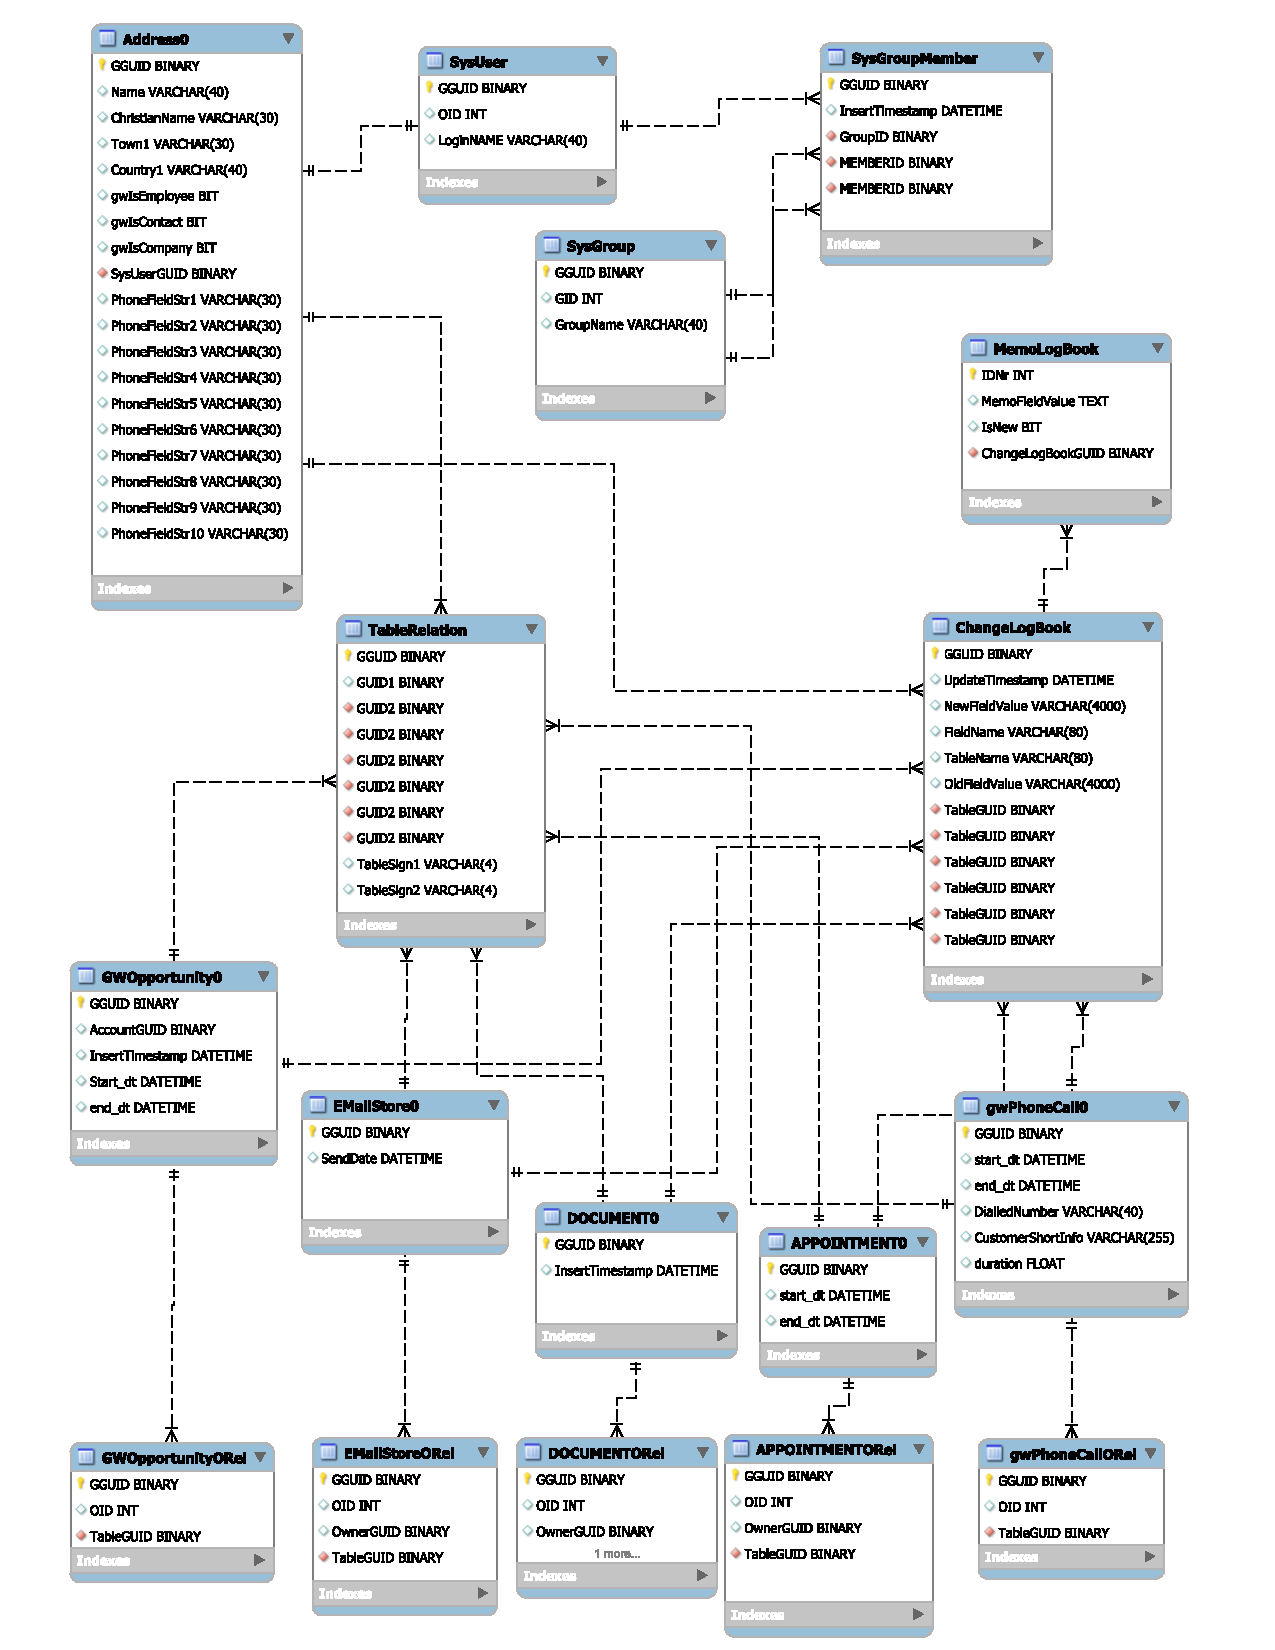
\includegraphics[width=1.0\textwidth]{pics/schema_alt.pdf}
	\caption{Auszug aus dem Schema des MSSQL 2008}
	\label{gw_schema_alt}
\end{figure}

Alle Informationen zu den Verkaufschancen finden sich in der Tabelle \textit{GWOpportunity0}. Die Spalte \textit{InsertTimestamp} wird zum Ermitteln des Erzeugungszeitpunktes benötigt. \textit{start\_dt} und \textit{end\_dt} legen den Zeitraum der Verkaufschance fest. Der Besitzer einer Verkaufschance wird über die Spalte \textit{AccountGUID} bestimmt. Mit den Tabellen \textit{EMailStore0}, \textit{Document0} \textit{Appointment0} und \textit{gwPhoneCall0} verhält es sich wie mit der Tabelle \textit{GWOpportunity0}. Bei der Tabelle\textit{EMailStore0} wird allerdings die Spalte \textit{SendDate} zur zeitlichen Einordnung verwendet. Eine weitere Besonderheit ist in der Spalte \textit{DialledNumber} der Tabelle \textit{gwPhoneCall0} vorhanden. Sie wird zum Vergleich mit der in der Adresse hinterlegten Telefonnummer benötigt. Um festzustellen, ob das Telefonat über einen Tag hinausging wird die Spalte \textit{duration} herangezogen.

Beziehungen lassen sich nicht nur aus der \textit{TableRelation} entnehmen, sondern auch aus den Tabellen die auf \textit{ORel} enden. In ihnen werden  Beziehungen aufbewahrt die durch Teilen von Zugriffsrechten entstanden sind. Jede dieser Tabellen enthält eine \textit{OID} bzw. \textit{GID}, die zur Bestimmung der beteiligten Personen dienen.

Eine Betrachtung basierend auf Zeitspannen impliziert die Veränderung von Zuständen und Konstellationen über die Zeit hinweg. Um diese Änderungen zu erfassen wird die Tabelle \textit{ChangeLogBook} benötigt. Die Spalte \textit{NewFieldValue} enthält die neuen Werte von Tupeln, wohingegen die Spalte \textit{OldFieldValue} den alten Wert besitzt. Die durch die Aktualisierung betroffene Spalte ist in der Spalte \textit{FieldName} hinterlegt. Der Name der betroffenen Tabelle ist der Spalte \textit{TableName} zu entnehmen. Die Referenzierung auf eine Tupel wird in der Spalte \textit{TableGUID} vorgenommen. Aus Gründen des Speicherplatzverbrauchs werden nur varchar Datentypen bei Zeichenfolgen verwendet. Varchar ist allerdings auf 4000 Zeichen limitiert. Falls Zeichenfolgen diese Grenze überschreiten, werden diese in der Tabelle \textit{MemoLogBook} abgelegt. Dort wird der Datentyp Text verwendet, der eine maximale Zeichenfolgenlänge von $2^{31}-1$ (2.147.483.647) erlaubt.